\chapter{Implementation}
\label{ch:Implementation}
This chapter explains the detailed implementation of the methods described in \autoref{ch:Methodology}. It covers the specific processes, experiments, and analyses conducted. This includes the practical steps taken to prepare images, apply distortions, extract features, and train the models to assess image quality in teledermatology. \par

\section{Image Selection and Labeling Process}
\label{sec:ImgSelectLabel}
This section describes the initial stages of the implementation, focusing on the selection and preparation of the image datasets used in the study. \par

\subsection{Image Filtering and Selection}
\label{sub:ImgFilterSelect}
The first step in preparing the images involves carefully choosing good quality pictures from the SCIN and Fitzpatrick17k datasets. This selection is done manually to ensure that each image is clear and useful for clinical purposes. The primary focus during selection is on images that are well-framed and free of any distortions that might affect their usefulness in diagnosis. \par
\vspace{\baselineskip}
\noindent
Each selected image is checked to ensure it is not blurred, as clear images are crucial for accurate diagnosis. Additionally, it is important that the images have proper lighting and true contrast, meaning they should not be too bright or too dark. Proper lighting and contrast help in accurately showing the skin’s condition. Lastly, the images must represent realistic skin tones and colors because accurate color representation is critical for correct diagnoses. Some pictures from the dataset are included in the appendix for reference (see Appendix).\todo{maybe include some pictures in appendix} \par

\subsection{Labeling of the Test Set}
\label{sub:LabelingTestSet}
The labeling process involves manually scoring 200 images from the SCIN dataset. Of these 200, around 50 are good quality images, which I wanted to represent in the test set as well. Each image is scored on a scale from 0 to 1 for each criterion, where 0 indicates no distortion and 1 indicates extreme distortion. This manual labeling is done using a custom Python script \footnote{src/create\_labels.ipynb} \todo{correct this later}, which displays each image and prompts the user to enter scores for each distortion criterion. The scores are collected in a structured format and stored in a JSON file for later analysis. \par
\vspace{\baselineskip}
\noindent
This structured approach ensures consistent and thorough evaluation of each image. I did the labeling myself, using an absolute categorical rating method as described in \autoref{sub:SubjectiveQualityAssessment}. This method is very time consuming and requires significant effort from the evaluator. My labeling process involved scoring 200 images on 7 criteria each, resulting in 1400 labels. To ensure accuracy and avoid rushing, I deliberately spread out the labeling over multiple sessions.\par
\noindent
\subsubsection{Visualization of Label Distribution for the Test Set}
\label{subsub:LabelDist}
To understand the distribution of labels and how often distortions occur across different criteria, see \autoref{fig:DistTestCriteria}. These histograms are useful for visualizing the prevalence and severity of distortions in the dataset. The histograms are plotted with 10 bins for each criterion, where the first bin indicates no distortion, and the remaining bins represent increasing levels of distortion severity for that type. \par
\begin{figure}[ht]
    \centering
    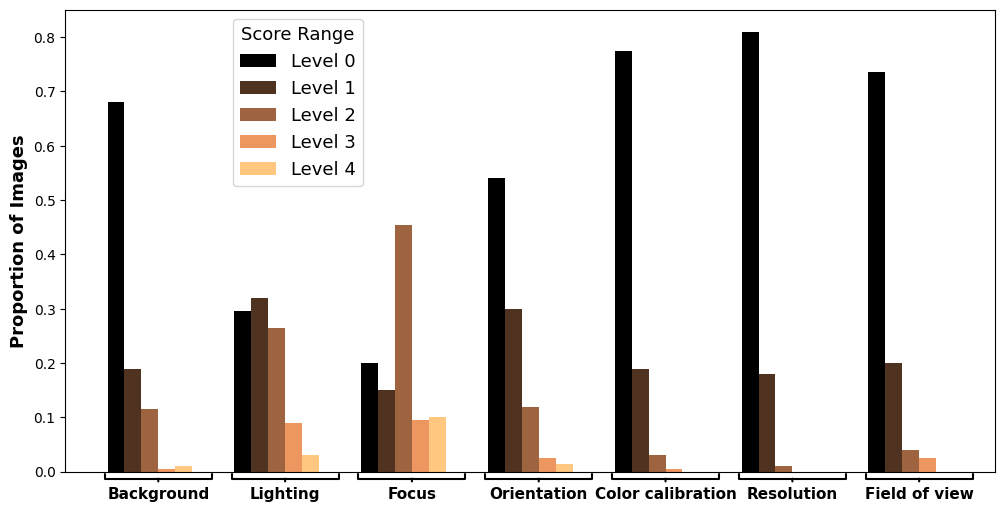
\includegraphics[keepaspectratio,width=15cm]{img/Distribution_test_criteria.png}
    \caption{Histograms showing the distribution of distortion scores for each quality criterion.}
    \label{fig:DistTestCriteria}
\end{figure}
\noindent
In \autoref{fig:DistTestCriteria} most criteria show a right-skewed distribution, indicating that higher levels of distortions are less common. This is evident in the criteria such as orientation, color calibration, background, resolution, and field of view. In contrast, the distributions for lighting and focus are more symmetrical, suggesting a more even spread of distortion severity levels. Since an image can have multiple distortions at once, it was difficult to separate them individually. For example, when an image is dark due to lighting issues, it becomes hard to judge other factors like focus, resolution, background, or color accuracy. These findings highlight the need to handle multiple distortions together during model training. They also point out the challenges in accurately labeling and assessing images that have several overlapping distortions. \par
\begin{figure}[ht]
    \centering
    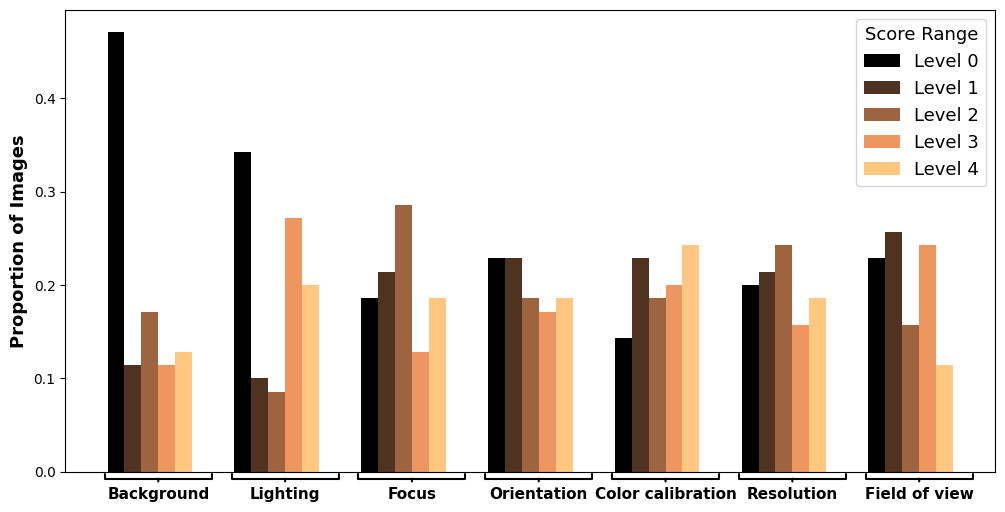
\includegraphics[keepaspectratio,width=15cm]{img/Distribution_test_criteria2.png}
    \caption{Histograms showing the distribution of distortion scores for each quality criterion.}
    \label{fig:DistTestCriteria2}
\end{figure}
\noindent
\section{Distortion Pipeline}
\label{sec:DistPipeline}
The distortion pipeline is central to simulating realistic image quality issues in teledermatology. Each quality criterion has multiple types of distortions, each having five levels of intensity, increasing in severity. All distortion types begin at zero, indicating no distortion applied, and progress to higher values that represent increasing levels of the specified distortion. Visual representations of the types of degradations at different ranges for each quality criterion are provided in \autoref{ch:Supplementary}.  \par

\subsection{Distortion Types}
\label{sub:DistTypes}
Here, each distortion type is briefly described, highlighting how they simulate different aspects of image degradation: \par
\begin{enumerate}
    \item Lighting:
        \begin{itemize}
            \item \textit{Brighten}: This operation increases the brightness of an image by applying color space transformations and adjustments, enhancing the overall visual intensity.
            \item \textit{Darken}: Similar to the brighten operation but reduces the visual intensity, making the image darker.
        \end{itemize}
    \item Focus:
        \begin{itemize}
            \item \textit{Gaussian blur}: Applies a Gaussian kernel to create a blurred effect, which softens the image by averaging the pixel values.
            \item \textit{Lens blur}: Uses a circular kernel to simulate the effect of a camera lens blur, causing a more uniform blur across the image.
            \item \textit{Motion blur}: Simulates the effect of motion, either from the camera or the subject, by applying a linear blur in a specified direction.
        \end{itemize}
    \item Orientation:
        \begin{itemize}
            \item \textit{Top perspective}: Alters the image to appear as if viewed from a higher angle, distorting the top part of the image.
            \item \textit{Bottom perspective}: Alters the image to appear as if viewed from a lower angle, distorting the bottom part of the image.
            \item \textit{Left perspective}: Alters the image to appear as if viewed from the left side, distorting the left part of the image.
            \item \textit{Right perspective}: Alters the image to appear as if viewed from the right side, distorting the right part of the image.
        \end{itemize}
    \item Color calibration:
        \begin{itemize}
            \item \textit{Color saturation 1}: Adjusts the saturation in the HSV color space, either increasing or decreasing the vividness of the colors.
            \item \textit{Color saturation 2}: Modifies the color channels in the LAB color space to change the saturation levels, affecting the color intensity.
        \end{itemize}
    \item Background:
        \begin{itemize}
            \item \textit{Color Block}: Uses skin segmentation to apply color block artifacts in the background, simulating background distortions and maintaining focus on the skin area.
        \end{itemize}
    \item Resolution:
        \begin{itemize}
            \item \textit{Change Resolution}: Alters the image resolution to simulate low-quality images by downsampling and then upsampling the image.
        \end{itemize}
    \item Field of view:
        \begin{itemize}
            \item \textit{Crop Image}: Crops the image to simulate different levels of field of view, reducing the visible area of the image.
        \end{itemize}
\end{enumerate}
\vspace{\baselineskip}
\noindent
The distortions for Lighting, Focus, and Color Calibration were adapted from the ARNIQA \autocite{ARNIQA} image degradation model, where they originally provided an extensive range of severity levels. I modified the severity levels to better fit real-world distortions commonly encountered in teledermatology. The rest of the distortions were designed based on my own observations of real-world image quality issues in teledermatology. \par

\section{Distortion Implementation Process}
\label{sec:DistProcess}

\begin{figure}[ht]
    \centering
    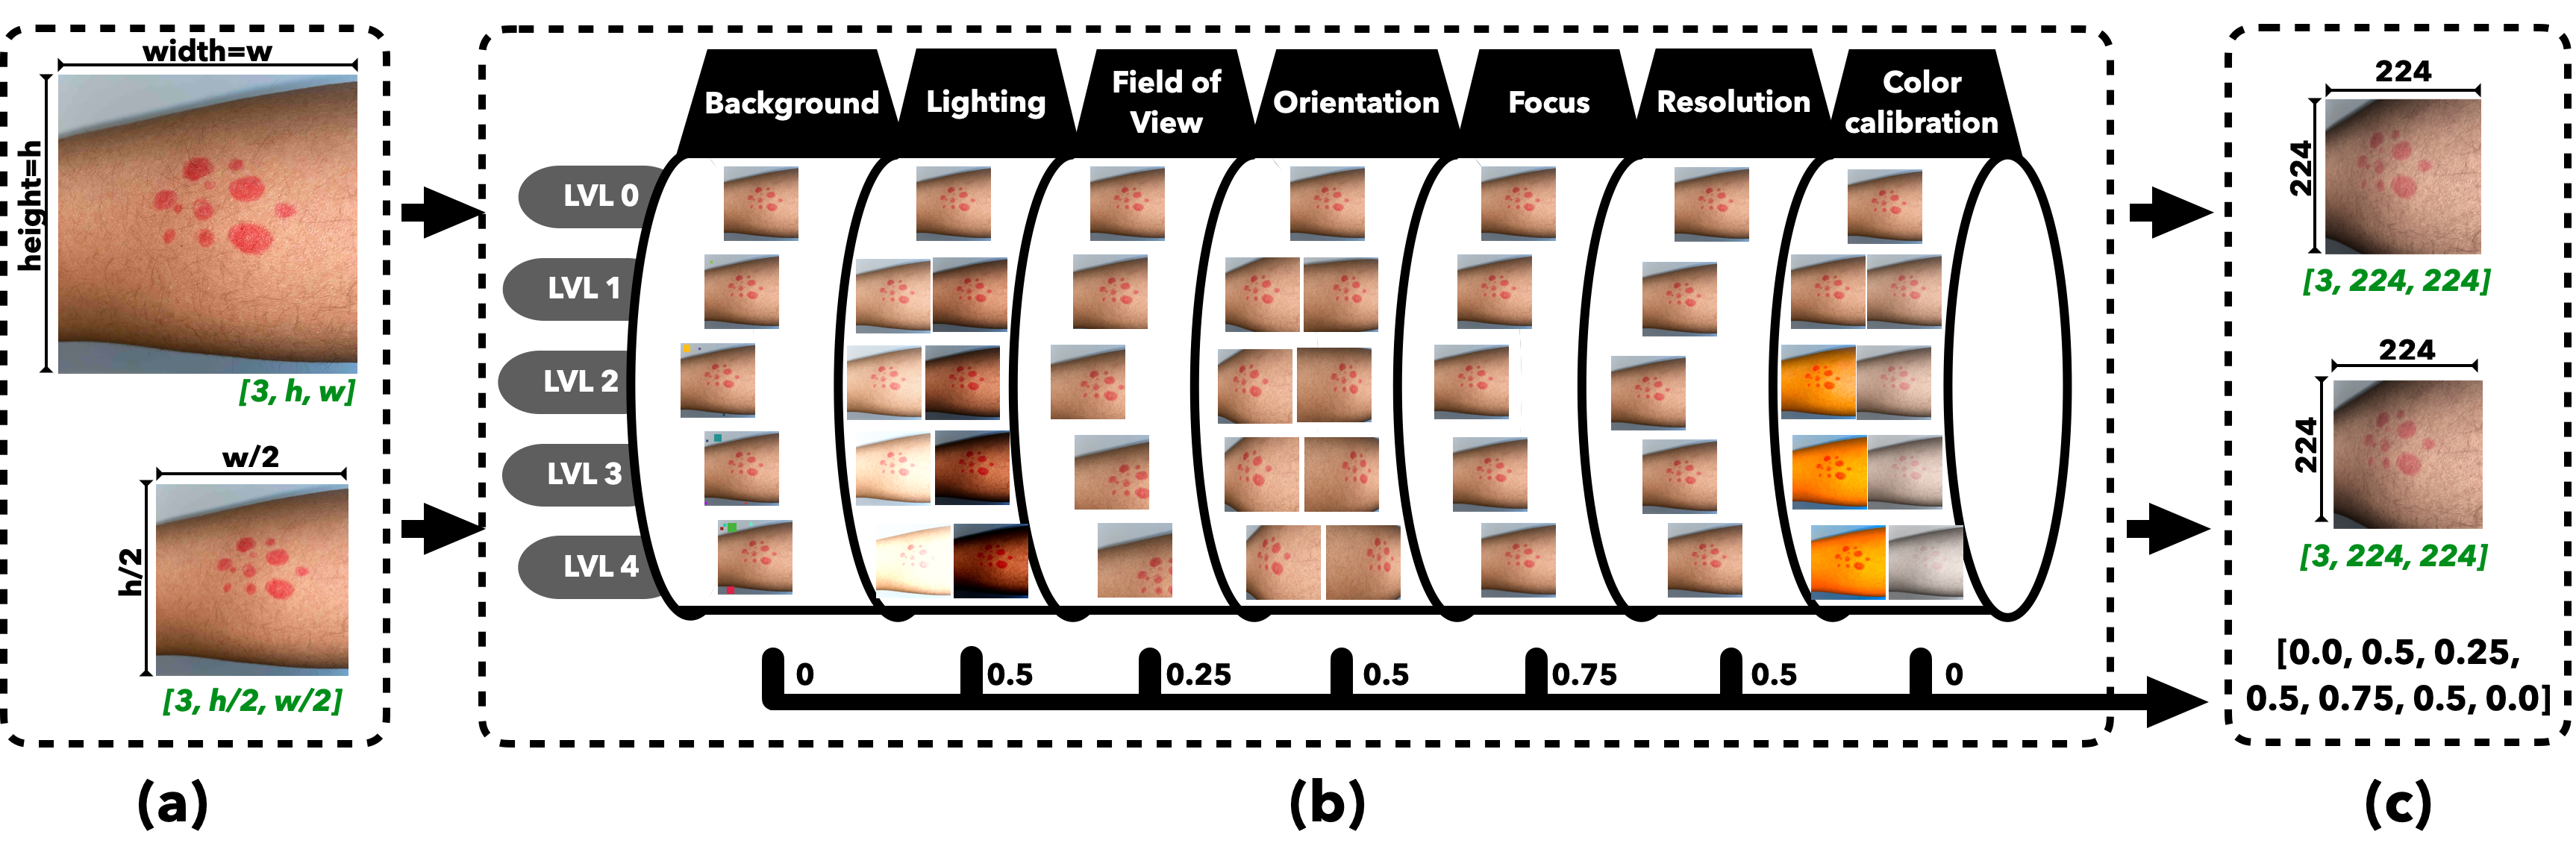
\includegraphics[keepaspectratio,width=15cm]{img/Distortion_pipeline.png}
    \caption{Distortion pipeline for generating training images with varying levels of distortion.}
    \label{fig:DistPipeline}
\end{figure}

The distortion implementation process involves several key steps to create a diverse and realistic set of distorted images, suitable for training and evaluating the image quality assessment model. \par
\vspace{\baselineskip}
\noindent
For each image, the RGB version is taken and a downsampled version of the image at half the resolution is created. This involves resizing the image to half its original dimensions to simulate lower resolution. Distortions are then applied in a specific sequence to ensure realistic simulation. The background distortion is applied first because it relies on the content of the undistorted image for skin segmentation. After that, other distortions are applied based on randomly chosen severity ranges. This ensures a variety of distortion levels across the dataset. \par
\vspace{\baselineskip}
\noindent
Once the distortions are applied, both the original and downsampled images are resized to 224x224 pixels to match the requirements of the SimCLR model from ARNIQA \autocite{ARNIQA}. Following resizing, both images are normalized using the mean and standard deviation values of the ImageNet dataset (mean=[0.485, 0.456, 0.406], std=[0.229, 0.224, 0.225]). This normalization step is crucial as it aligns with the preprocessing used in the pretrained SimCLR model. \par
\vspace{\baselineskip}
\noindent
The severity of each applied distortion is mapped to a value between 0 and 1. This is done by taking the minimum and maximum possible values of the distortion and scaling the actual distortion value within this range. This standardized representation allows for consistent training and evaluation of the model later on. \par
\vspace{\baselineskip}
\noindent
This process can generate 3'750'000 possible combinations of distorted images because of the random selection of distortion types and severity levels. This highlights the robustness and adaptability of the pipeline. By following this detailed and structured approach, the distortion pipeline effectively simulates a wide range of real-world image quality issues in teledermatology, providing a comprehensive dataset for training and evaluating the image quality assessment model. \par

\begin{figure}[ht]
    \centering
    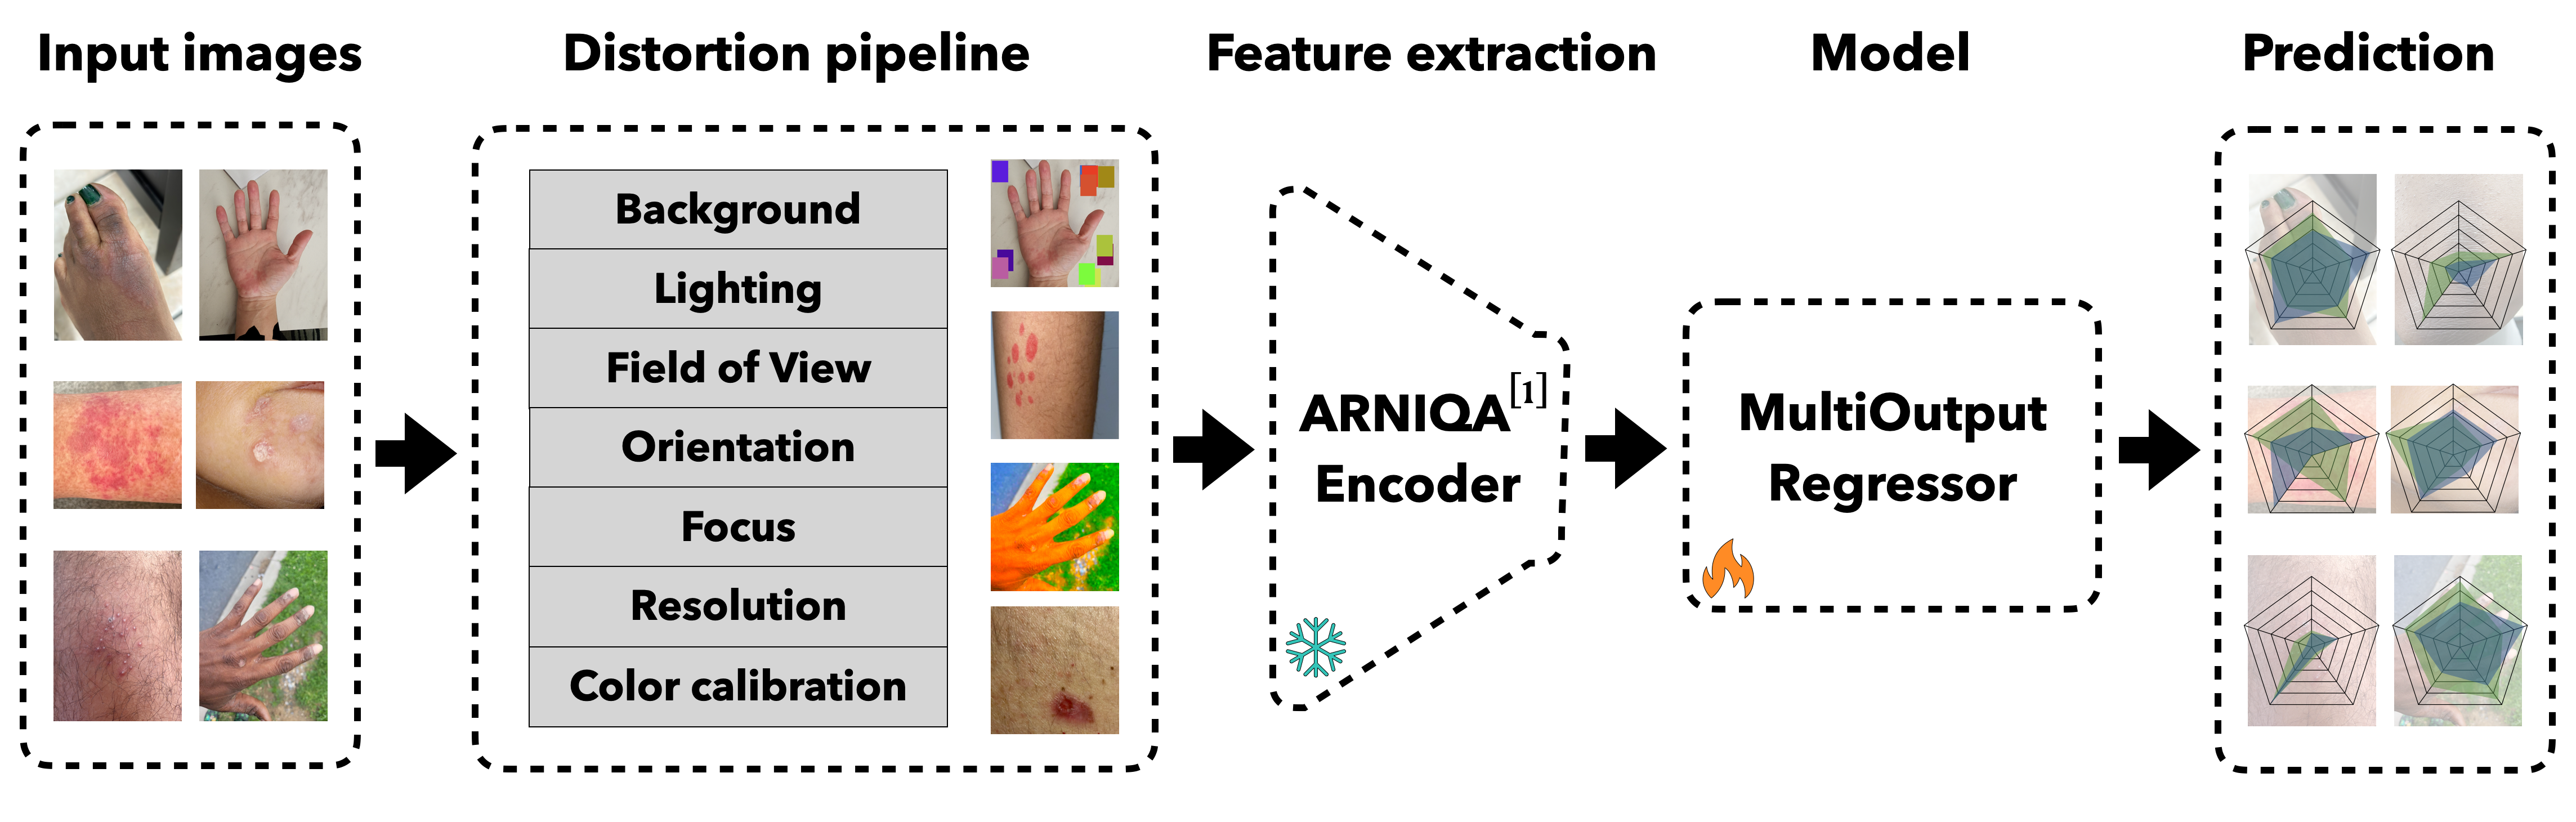
\includegraphics[keepaspectratio,width=15cm]{img/Architecture.png}
    \caption{Architecture.}
    \label{fig:Architecture}
\end{figure}

\section{Feature Extraction with SimCLR}
\label{sec:FeatureExtraction}
After creating the distortions and their half-scaled versions with mapped labels, the next step is to use the pretrained model from ARNIQA, loaded via \textit{torch.hub}, which uses the SimCLR framework. This framework, a self-supervised learning method, helps capture the patterns of distortions in the images rather than their content. This approach is crucial because it allows the model to focus on the actual distortions affecting image quality, making the assessment more accurate. \par
\vspace{\baselineskip}
\noindent
The pretrained model has already learned useful representations from a large dataset, which can be transferred to our specific task. This transfer learning approach saves time and computational resources while enhancing the model's performance. By using SimCLR, the framework generates feature vectors that represent the distortion patterns in the images. This dual-input method, which includes both the original and downscaled images, ensures that the model effectively learns to distinguish between different levels of distortion.\par
\vspace{\baselineskip}
\noindent
The extracted features from both the original and downscaled images are then combined and used to train the final image quality assessment model with the corresponding generated distortion severity labels. \par

\section{Model Selection and Training}
\label{sec:ModelTraining}
To train the model, I began by splitting the images into a training set (75\%) and a validation set (25\%). For this task, I experimented with three different models: a multioutput XGBRegressor, an XGBClassifier, and an MLP Regressor. These models were chosen because to their strengths in handling complex, nonlinear relationships and their flexibility in output formats. \par
\vspace{\baselineskip}
\noindent
The XGBRegressor and XGBClassifier were selected for their robustness and efficiency. XGBoost is well-known for its ability to handle large datasets and capture complex patterns effectively. The regressor was used to predict continuous severity scores for each quality criterion, while the classifier was used to categorize these scores into predefined severity levels. Additionally, the MLP Regressor, a type of neural network, was chosen for its ability to learn intricate patterns through its deep network structure, making it particularly suitable for regression tasks involving multiple outputs. \par

\subsection{Performance Metrics}
\label{sub:PerfMetrics}


\section{Model Testing}
\label{sec:ModelTesting}
The final model is tested against the labeled test set to evaluate its performance in real-world scenarios. Plots illustrating the model’s performance across various quality criteria will be shown, highlighting areas where the model performs well or where there is significant variance, indicating uncertainty in quality assessment. \par
\vspace{\baselineskip}
\noindent

\subsection{Testing with Labeled Test Set}
\label{sub:TestLabeledSet}